\documentclass[12pt]{article}


\usepackage{amssymb}
\usepackage{amsmath}
\usepackage{fullpage}
\usepackage{epsfig}
\usepackage{epstopdf}
\everymath{\displaystyle}
\usepackage{enumerate}



\begin{document}

\begin{center}
\underline{\LARGE{Cylindrical \& Spherical Coordinates}}
\end{center}

\noindent SUGGESTED REFERENCE MATERIAL:

\bigskip

\noindent As you work through the problems listed below, you should reference Chapter 11.8 of the recommended textbook (or the equivalent chapter in your alternative textbook/online resource) and your lecture notes.

\bigskip

\noindent EXPECTED SKILLS:

\begin{itemize}

\item Be able to convert between rectangular, cylindrical, and spherical coordinates (Table 11.8.1). 

\item Be able describe simple surfaces in terms of cylindrical and spherical coordinates (Table 11.8.2).

\end{itemize}

\noindent PRACTICE PROBLEMS:

\medskip

\begin{enumerate}

\item Consider the point $(r,\theta,z)=\left(2, \frac{\pi}{2}, 1\right)$ in cylindrical coordinates.

\begin{enumerate}

\item Convert this point to rectangular coordiinates.

\includegraphics[scale=0.5]{start.pdf}
{{$(x,y,z)=(0,2,1)$}}
\includegraphics[scale=0.5]{end.pdf}


\item Convert this point to spherical coordinates.

\includegraphics[scale=0.5]{start.pdf}
{{$(\rho, \theta, \phi)=\left(\sqrt{5}, \frac{\pi}{2}, \cos^{-1}\frac{1}{\sqrt{5}}\right)$}}
\includegraphics[scale=0.5]{end.pdf}


\end{enumerate}

\item Consider the point $(r,\theta,z)=\left(1, \frac{\pi}{4}, -4\right)$ in cylindrical coordinates.

\begin{enumerate}

\item Convert this point to rectangular coordiinates.

\includegraphics[scale=0.5]{start.pdf}
{{$(x,y,z)=\left(\frac{\sqrt{2}}{2},\frac{\sqrt{2}}{2},-4\right)$}}
\includegraphics[scale=0.5]{end.pdf}


\item Convert this point to spherical coordinates.

\includegraphics[scale=0.5]{start.pdf}
{{$(\rho, \theta, \phi)=\left(\sqrt{17}, \frac{\pi}{4}, \cos^{-1}\left(-\frac{4}{\sqrt{17}}\right)\right)$}}
\includegraphics[scale=0.5]{end.pdf}


\end{enumerate}

\item Consider the point $(\rho,\theta,\phi)=\left(5, \frac{\pi}{3}, \frac{2\pi}{3}\right)$ in spherical coordinates.

\begin{enumerate}

\item Convert this point to rectangular coordiinates.

\includegraphics[scale=0.5]{start.pdf}
{{$(x,y,z)=\left(\frac{5\sqrt{3}}{4},\frac{15}{4},-\frac{5}{2}\right)$}}
\includegraphics[scale=0.5]{end.pdf}


\item Convert this point to cylindrical coordinates.

\includegraphics[scale=0.5]{start.pdf}
{{$(r, \theta, z)=\left(\frac{5\sqrt{3}}{2}, \frac{\pi}{3}, -\frac{5}{2}\right)$}}
\includegraphics[scale=0.5]{end.pdf}


\end{enumerate}

\item Consider the point $(x,y,z)=\left(1, -\sqrt{3}, -2\right)$ in rectangular coordinates.

\begin{enumerate}

\item Convert this point to cylindrical coordiinates.

\includegraphics[scale=0.5]{start.pdf}
{{$(r, \theta, z)=\left(2, \frac{5\pi}{3}, -2\right)$}}
\includegraphics[scale=0.5]{end.pdf}


\item Convert this point to spherical coordinates.

\includegraphics[scale=0.5]{start.pdf}
{{$(\rho, \theta, \phi)=\left(\sqrt{8}, \frac{5\pi}{3}, \frac{3\pi}{4}\right)$}}
\includegraphics[scale=0.5]{end.pdf}


\end{enumerate}

\end{enumerate}

\newpage

\noindent {\bf For problems 5-10, each of the given surfaces is expressed in rectangular coordinates.  Express the equation of the surface in (a) cylindrical coordinates and (b) spherical coordinates.}

\begin{enumerate}
\setcounter{enumi}{4}

\item $x^2+y^2+z^2=16$

\includegraphics[scale=0.5]{start.pdf}
{{(a)$r^2+z^2=16$; (b) $\rho=4$}}
\includegraphics[scale=0.5]{end.pdf}


\item $x^2+y^2+z^2=3z$

\includegraphics[scale=0.5]{start.pdf}
{{(a)$r^2+z^2=3z$; (b) $\rho=3\cos{\phi}$}}
\includegraphics[scale=0.5]{end.pdf}


\item $z=\sqrt{2x^2+2y^2}$

\includegraphics[scale=0.5]{start.pdf}
{{(a)$z=\sqrt{2}r$; (b) $\phi=\cos^{-1}\left(\frac{2}{\sqrt{6}}\right)$}}
\includegraphics[scale=0.5]{end.pdf}


\item $x^2+y^2=9$

\includegraphics[scale=0.5]{start.pdf}
{{(a)$r=3$; (b) $\rho\sin{\phi}=3$}}
\includegraphics[scale=0.5]{end.pdf}


\item $x+3y+5z=4$

\includegraphics[scale=0.5]{start.pdf}
{{(a)$r\cos{\theta}+3r\sin{\theta}+5z=4$; (b) $\rho\cos{\theta}\sin{\phi}+3\rho\sin{\theta}\sin{\phi}+5\rho\cos{\phi}=4$}}
\includegraphics[scale=0.5]{end.pdf}


\item $z=2$

\includegraphics[scale=0.5]{start.pdf}
{{(a)$z=2$; (b) $\rho\cos{\phi}=2$}}
\includegraphics[scale=0.5]{end.pdf}


\end{enumerate}

\noindent {\bf For problems 11-15, each of the given surfaces is expressed in cylindrical coordinates.  Express the equation of the surface in rectangular coordinates.}

\begin{enumerate}
\setcounter{enumi}{10}

\item $r=5$

\includegraphics[scale=0.5]{start.pdf}
{{$x^2+y^2=25$}}
\includegraphics[scale=0.5]{end.pdf}


\item $\theta=\frac{\pi}{2}$

\includegraphics[scale=0.5]{start.pdf}
{{$x=0$, where $y \geq 0$}}
\includegraphics[scale=0.5]{end.pdf}


\item $r=6\sin{\theta}$

\includegraphics[scale=0.5]{start.pdf}
{{$x^2+(y-3)^2=9$}}
\includegraphics[scale=0.5]{end.pdf}


\item $z=r\sin{\theta}$

\includegraphics[scale=0.5]{start.pdf}
{{$z=y$}}
\includegraphics[scale=0.5]{end.pdf}


\item $r^2\sin{2\theta}=z$

\includegraphics[scale=0.5]{start.pdf}
{{$z=2xy$}}
\includegraphics[scale=0.5]{end.pdf}


\end{enumerate}

\noindent {\bf For problems 16-19, each of the given surfaces is expressed in spherical coordinates.  Express the equation of the surface in rectangular coordinates.}

\begin{enumerate}
\setcounter{enumi}{15}

\item $\rho=4$

\includegraphics[scale=0.5]{start.pdf}
{{$x^2+y^2+z^2=16$}}
\includegraphics[scale=0.5]{end.pdf}


\item $\phi=\frac{\pi}{3}$

\includegraphics[scale=0.5]{start.pdf}
{{$z=\frac{1}{\sqrt{3}}\sqrt{x^2+y^2}$}}
\includegraphics[scale=0.5]{end.pdf}


\item $\rho=4\cos{\phi}$

\includegraphics[scale=0.5]{start.pdf}
{{$x^2+y^2+(z-2)^2=4$}}
\includegraphics[scale=0.5]{end.pdf}


\item $\rho=3\sec{\phi}$

\includegraphics[scale=0.5]{start.pdf}
{{$z=3$}}
\includegraphics[scale=0.5]{end.pdf}


\end{enumerate}


\noindent {\bf For problems 20-21, describe in words all points in 3-space which satisfy the given inequalities.}

\begin{enumerate}
\setcounter{enumi}{19}

\item In cylindrical coordinates: $\left\{(r,\theta,z): 0 \leq r \leq 2, 0 \leq \theta \leq \frac{\pi}{3}, 0 \leq z \leq 1\right\}$

\includegraphics[scale=0.5]{start.pdf}
{{{1\linewidth}{All points in the first octant which are on or inside of the circular cylinder $x^2+y^2=4$ between the planes $z=0$, $z=1$, $y=0$ and $y=\sqrt{3}x$.
\begin{center}
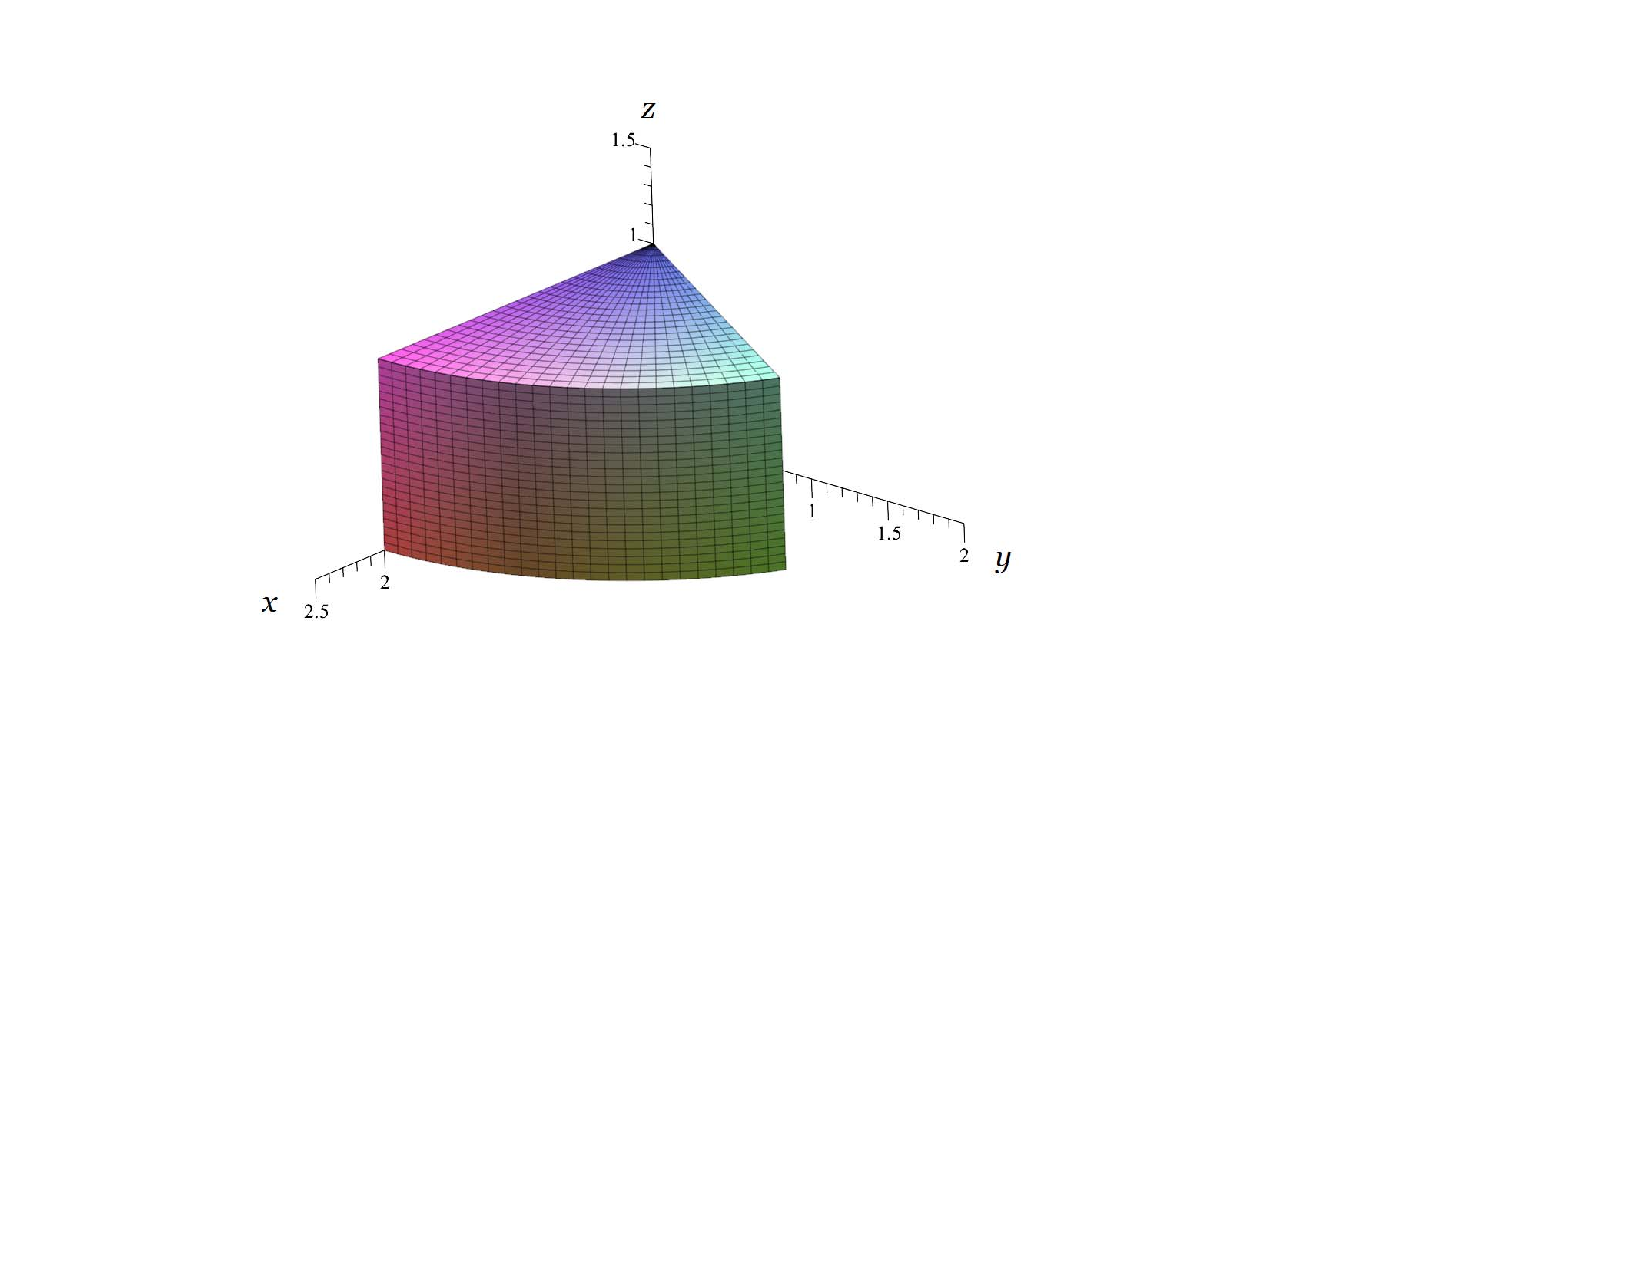
\includegraphics[scale=0.4]{describe1.pdf}
\end{center}}}}
\includegraphics[scale=0.5]{end.pdf}


\item In spherical coordinates: $\left\{(\rho,\theta,\phi): 1 \leq \rho \leq 3, 0 \leq \theta \leq \frac{\pi}{2}, 0 \leq \phi \leq \frac{\pi}{4}\right\}$

\includegraphics[scale=0.5]{start.pdf}
{{{1\linewidth}{All points in the first octant which are on and between the spheres $x^2+y^2+z^2=1$ and $x^2+y^2+z^2=9$, on and between the planes $x=0$ and $y=0$, and on or within the cone $z=\sqrt{x^2+y^2}$.}}}
\includegraphics[scale=0.5]{end.pdf}


\end{enumerate}


\end{document}